
\documentclass[11pt,a4paper,openany]{report}
\usepackage[T1]{fontenc}
\usepackage[utf8]{inputenc}
\usepackage{lmodern}
\usepackage{microtype}
\usepackage{amsmath,amssymb,amsthm,mathtools,bm}
\usepackage{booktabs,array,longtable,tabularx}
\usepackage{xcolor}
\usepackage[margin=22mm,headheight=23pt]{geometry}
\usepackage{enumitem}
\usepackage{fancyhdr}
\usepackage{fancyvrb}
\usepackage{graphicx}
\usepackage{url}
\usepackage{xurl}
\usepackage{hyperref}
\definecolor{finblue}{HTML}{1F5A99}
\definecolor{fingreen}{HTML}{19733A}
\definecolor{finorange}{HTML}{D55E00}
\definecolor{finred}{HTML}{A61B1B}
\definecolor{finviolet}{HTML}{6A3D9A}
\definecolor{fingray}{HTML}{4D4D4D}

\hypersetup{
  unicode=true,
  colorlinks=true,
  linkcolor=finblue,
  citecolor=fingreen,
  urlcolor=finblue,
  pdftitle={FIN Research Programs P411--P427},
  pdfauthor={Krzysztof Żuchowski},
  pdfsubject={Formal cosine boundary, simultaneous contact geometry, erasure-aware discrimination, and operational reference resources},
  pdfkeywords={FIN, Lean, Taylor theorem, KKT, signed moment problem, nonlinear recurrence, photonic identifiability, quantum discrimination, erasure, Jordan sampling, phase reference, orientation torsor, scale section}
}
\pagestyle{fancy}
\fancyhf{}
\fancyhead[L]{\small FIN Programs P411--P427}
\fancyhead[R]{\small Release 10.35}
\fancyfoot[C]{\thepage}

\setlength{\parindent}{0pt}
\setlength{\parskip}{0.55em}
\setlist{nosep,leftmargin=2em}
\setcounter{tocdepth}{2}
\setcounter{secnumdepth}{3}
\emergencystretch=3em
\newcommand{\one}{\bm 1}
\newcommand{\C}{\mathbb C}
\newcommand{\R}{\mathbb R}
\newcommand{\Z}{\mathbb Z}
\newcommand{\statusProven}{\textcolor{fingreen}{[Proven]}}
\newcommand{\statusStrong}{\textcolor{finblue}{[Strong evidence]}}
\newcommand{\statusModerate}{\textcolor{finviolet}{[Moderate evidence]}}
\newcommand{\statusWeak}{\textcolor{fingray}{[Weak evidence]}}
\newcommand{\statusSpeculative}{\textcolor{finorange}{[Speculative]}}
\newcommand{\statusRefuted}{\textcolor{finred}{[Refuted]}}

\begin{document}
\hypersetup{pageanchor=false}
\begin{titlepage}
\centering
\vspace*{7mm}
{\Large\bfseries FIN --- Release 10.35\par}
\vspace{9mm}
{\Huge\bfseries Research Programs P411--P427\par}
\vspace{6mm}
{\Large Formal cosine boundary, simultaneous contact geometry,\\
erasure-aware discrimination, and operational reference resources\par}
\vspace{13mm}
{\Large Krzysztof \.Zuchowski\par}
\vspace{2mm}
{\normalsize Independent Researcher --- Fractal Information Theory Project\par}
\vspace{2mm}
{\normalsize ORCID:
\href{https://orcid.org/0009-0002-0909-3613}{0009-0002-0909-3613}\par}
\vspace{7mm}
{\large 31 July 2026\par}
{\normalsize Publication --- Preprint; Version 1.0.0\par}
\vfill
\begin{minipage}{0.92\textwidth}
\small
\textbf{Constructive operational result.}
The heralded-erasure-aware symmetric code improves both product and GHZ
baselines in all 16 declared noise cells, with maximum gain approximately
\(0.02694\).

\medskip
\textbf{Exact estimator result.}
\[
q_i^\star\propto |w_i|
\sqrt{\sum_{k=0}^{11}x_i^{2k}},
\]
reducing the declared twelve-moment variance by approximately \(11.57\%\).

\medskip
No non-premise selector, dimensional source, laboratory record, complete
legacy-to-strict bridge, role transfer, Standard Model, gravity, or
Theory-of-Everything closure is claimed.

\medskip
\textbf{Repository.}
\url{https://github.com/hyconiek/Fractal-Nadsoliton-Theory}

\textbf{License.} CC BY 4.0.
\end{minipage}
\vfill
\end{titlepage}
\hypersetup{pageanchor=true}
\pagenumbering{roman}
\chapter*{Publication statement}
\addcontentsline{toc}{chapter}{Publication statement}
This monograph reports every executed Program P411--P427 and recommends
Programs P428--P444. Mathematical proof, numerical evidence, conditional
operational structure, and absent external evidence are kept distinct.

\tableofcontents
\clearpage
\pagenumbering{arabic}

\chapter*{Confidence convention}
\addcontentsline{toc}{chapter}{Confidence convention}

\begin{center}
\begingroup\small
\setlength{\tabcolsep}{2.5pt}
\renewcommand{\arraystretch}{1.16}
\begin{longtable}{@{}p{0.420\textwidth}p{0.420\textwidth}@{}}
\toprule
\textbf{Label} & \textbf{Meaning} \\
\midrule
\endhead
\textbf{\statusProven{}} & Mathematical proof, exact arithmetic, proof-kernel result, or exhaustive finite computation \\
\textbf{\statusStrong{}} & Reproducible bounded/\allowbreak{}high-precision computation with explicit limitations \\
\textbf{\statusModerate{}} & Local or model-dependent numerical evidence \\
\textbf{[Conditional]} & Requires a named state, reference, clock, apparatus law, standard, or axiom \\
\textbf{\statusRefuted{}} & The declared proposition fails in its stated class \\
\textbf{[Blocked by external evidence]} & Independent hardware, data, custody, calibration, or unblinding is required \\
\bottomrule
\end{longtable}
\endgroup
\end{center}

\chapter{Scope and binding guardrails}

\section{The two kernels are not interchangeable}

The historical intermediate kernel is

\[
K_{\rm legacy,ont}(d)
=4\ln2\,
\frac{\cos(\pi d/4+\pi/6)}{1+0.01d},
\]

whereas the strict working kernel is

\[
K_{\rm strict,gate}(d)
=\frac{\cos((743/4000)d+13/80)}{1+d^{9/5}}.
\]

P414 concerns only a proposed mathematical source for the target-defined attenuation completion atom. It does not derive strict amplitude, phase, frequency, compression exponent, or physical meaning from the legacy kernel. No legacy electroweak, electromagnetic, or gravity-hierarchy formula is transported to the strict kernel.

\section{Operator duality remains mathematical}

For the strict finite generator

\[
A=sI-W,
\]

the same self-adjoint operator generates

\[
U_t=e^{-itA},
\qquad
P_t=e^{-tA}.
\]

This wave/\allowbreak{}heat duality is a consequence of spectral functional calculus. It does not choose a physical state, clock, environment, apparatus, detector, measurement record, or observer. The noisy channels used below are declared operational models added around the operator.

\section{Statements deliberately withheld}

This report does not claim:

\begin{itemize}
\item 
discharge of QW-2191;

\item 
a strict internal orientation or phase-origin selector;

\item 
a source-independent legacy-to-strict completion;

\item 
a canonical unit of action, time, length, mass, or energy;

\item 
that a laboratory realizes twelve FIN basis states or a vertex POVM;

\item 
transfer of the historical legacy physical roles;

\item 
a Standard Model, gravitational theory, total physical action, or Theory of Everything.

\end{itemize}

\chapter{Executive result table}

\begin{center}
\begingroup\small
\setlength{\tabcolsep}{2.5pt}
\renewcommand{\arraystretch}{1.16}
\begin{longtable}{@{}p{0.138\textwidth}p{0.403\textwidth}p{0.318\textwidth}@{}}
\toprule
\textbf{Program} & \textbf{Result} & \textbf{Status} \\
\midrule
\endhead
P411 & Exact rational Taylor algorithm for twelve phases checked by Lean & \statusProven{}; analytic cosine bridge open \\
P412 & Simultaneous 25-equation seven-contact candidate & \statusStrong{}; interval uniqueness open \\
P413 & Formal transcendence dependency isolated & [Proven interface]; LW library absent \\
P414 & One normalized nonlinear damping recurrence excluded & [Refuted source class] \\
P415 & Nine sampled 132-direction photonic Jacobians full rank & \statusStrong{}; global theorem open \\
P416 & Independent photonic pilot absent & [Blocked] \\
P417 & Optimized noisy parallel lower bounds and explicit gaps & \statusStrong{}; SDP dual open \\
P418 & Erasure-aware symmetric code improves product/\allowbreak{}GHZ in 16/\allowbreak{}16 cells & \statusStrong{} \\
P419 & Twelve-mode one-use optimization collapses to extremal pair on grid & \statusStrong{}; adaptive theorem open \\
P420 & Traceable clock anchor absent & [Blocked] \\
P421 & External P403/\allowbreak{}JSR execution absent & [Blocked] \\
P422 & Variance-optimal twelve-moment JSR sampler & \statusProven{} \\
P423 & Reference-frame conversion ledger; free coherence excluded & \statusProven{}/\allowbreak{}[Conditional] \\
P424 & Nonzero oriented record; selector promotion fails & \statusProven{}/\allowbreak{}\statusRefuted{} \\
P425 & Three conditional scale sections inequivalent & [Proven in declared coordinate] \\
P426 & QW/\allowbreak{}standards/\allowbreak{}reservoir admission absent & [Blocked] \\
P427 & Electroweak blind transfer test inadmissible & [Blocked] \\
\bottomrule
\end{longtable}
\endgroup
\end{center}

\chapter{P411 --- Taylor trust lattice}

\section{Frozen rational phases}

For integer distances \(d=0,\ldots,11\), define

\[
x_d=\frac{743d+650}{4000}.
\]

The strict moments use \(\cos x_d\). Define the exact rational sums

\[
S_n(x)=\sum_{k=0}^{n}\frac{(-1)^kx^{2k}}{(2k)!}.
\]

The generated Lean source independently evaluates

\[
L_d=S_{21}(x_d),
\qquad
U_d=S_{20}(x_d)
\]

and proves for every listed phase

\[
L_d<U_d,
\qquad
U_d-L_d<10^{-30}.
\]

The maximum exact rational width is

\[
1.9128718517\times10^{-37}.
\]

\section{Exact trust boundary}

The following distinction is essential.

\begin{center}
\begingroup\small
\setlength{\tabcolsep}{2.5pt}
\renewcommand{\arraystretch}{1.16}
\begin{longtable}{@{}p{0.420\textwidth}p{0.420\textwidth}@{}}
\toprule
\textbf{Component} & \textbf{Status} \\
\midrule
\endhead
Factorial recursion & Lean computed \\
Rational exponentiation & Lean computed \\
Alternating sums & Lean computed \\
Ordering and width & Lean proved by native decision \\
Real cosine object & Not present in dependency-free file \\
Alternating Taylor remainder theorem for cosine & Named external analytic bridge \\
\bottomrule
\end{longtable}
\endgroup
\end{center}

Thus P411 is not a complete formalization of real trigonometric analysis. It is a complete reflection of the exact rational arithmetic used once the standard analytic remainder theorem is provided.

\section{Falsification condition}

P411 would be invalidated as a cosine enclosure if the imported analytic bridge were applied outside its domain or with reversed parity. The file prevents this from becoming invisible by typing it as a separate premise.

\chapter{P412 --- simultaneous contact reconstruction}

\section{Why P395 was not the final optimizer}

P395 established that the frozen P366 primal and P380 dual were near-contact but had strictly positive slack at every primal atom. Complementary slackness therefore forbids treating that frozen pair as the exact optimal pair.

P412 instead solves primal moments, dual contact equations, and stationarity simultaneously.

\section{Unknowns and equations}

The 25 unknowns are:

\begin{itemize}
\item 
six interior atom positions;

\item 
seven signed weights;

\item 
twelve power-basis coefficients of a degree-eleven dual polynomial.

\end{itemize}

The equations are:

\begin{itemize}
\item 
twelve moment equalities;

\item 
seven contact equalities;

\item 
six interior derivative equalities.

\end{itemize}

The contact pattern is

\[
(-1,0,0,0,0,-1,0).
\]

The corresponding sign pattern is

\[
(-,+,+,+,+,-,+).
\]

\section{Candidate solution}

The nodes are approximately

\[
\begin{aligned}
&0.0198263786851,\quad0.1294227962491,\quad0.2950442572391,\\
&0.5266923563528,\quad0.8140632145104,\quad0.9418448480174,\quad1.
\end{aligned}
\]

The objective is

\[
\mathcal N_{\rm osc}^{\rm KKT}
=0.7073534677231137\ldots.
\]

This lies inside the Release-10.33 certified interval

\[
0.7073534379053974
\le\mathcal N_{\rm osc}
\le0.7073534683998260.
\]

\section{Why the status is not "Proven"}

The largest high-precision residual is approximately \(3.42\times10^{-28}\), but the numerical Jacobian has smallest singular value about \(4.99\times10^{-13}\) and condition number about \(2.73\times10^{15}\). This is a severely ill-conditioned system. A 25-variable interval Krawczyk or radii-polynomial certificate is required before local existence and uniqueness can be asserted. Global dual feasibility must then be checked by exact Bernstein subdivision.

\begin{figure}[htbp]
\centering
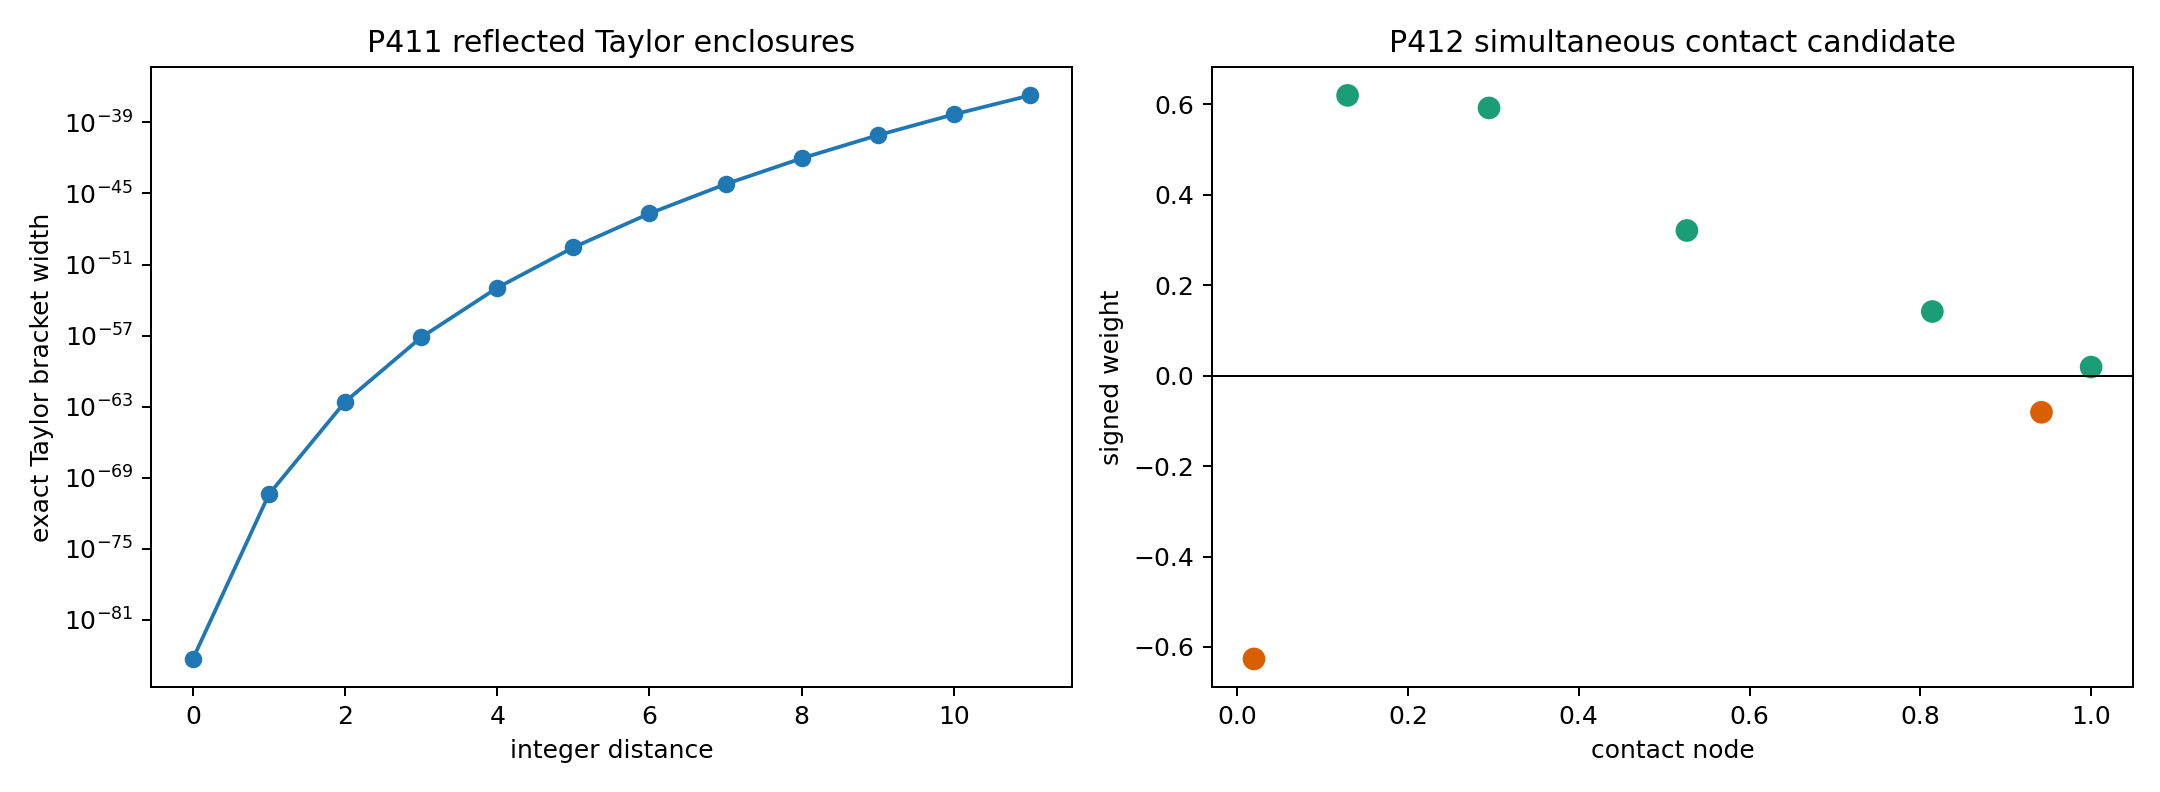
\includegraphics[width=0.97\textwidth]{FIN_Programs_411_427_Figures/p411_p412_formal_contact.png}
\caption{Exact reflected Taylor widths and the simultaneous seven-contact KKT candidate.}
\end{figure}

\chapter{P413 --- transcendence provider boundary}

P381 proved global injectivity of the strict radial law on \(\mathbb N_0\) using Lindemann--Weierstrass. P413 records the proof dependency inside Lean:

\[
K(d)=K(e),\quad d\ne e
\Longrightarrow
\sum_{j=1}^{4}a_j e^{\alpha_j}=0,
\]

where the coefficients are algebraic, the four exponents are distinct algebraic numbers, and the coefficient vector is nonzero.

The local source compiles the contradiction after receiving the exponential independence premise. It does not replace transcendence theory by an axiom of FIN; it makes the library boundary inspectable.

\chapter{P414 --- nonlinear damping-source falsification}

\section{Candidate flow}

The tested class is the normalized nonlinear flow

\[
R_\gamma(c)=\frac{c}{1+\gamma c},
\qquad c_{d+1}=R_\gamma(c_d),
\qquad c_0=1.
\]

It has the closed orbit

\[
c_d=\frac{1}{1+\gamma d}.
\]

This class is nonlinear in the state and strictly broader than the multiplicative-character class excluded by P397.

\section{Exact obstruction}

The target completion satisfies

\[
C_{\rm damp}(1)=\frac{101}{200}.
\]

Therefore the recurrence would require

\[
\gamma=\frac{99}{101}.
\]

It then predicts

\[
c_2=\frac{101}{299}.
\]

Equality with \(C_{\rm damp}(2)\) would force

\[
2^{4/5}=\frac{10199}{10100}.
\]

Raising to the fifth power gives the false integer equality

\[
10199^5=16\,10100^5,
\]

whose exact defect is

\[
-1571262110836960349001.
\]

The recurrence class is therefore rigorously excluded. Fractional memory, subordination, operator-valued flow, and state-dependent source classes are not excluded.

\chapter{P415--P416 --- photonic quotient frontier}

\section{Sampled regularity atlas}

The 66-component Givens mesh has 132 declared loss/\allowbreak{}phase coordinates. P415 evaluates the complex-transfer Jacobian at the origin and eight frozen random points in the bounded chart

\[
\ell_j\in[0,0.03],
\qquad
\varphi_j\in[-0.1,0.1].
\]

All nine numerical Jacobians have rank 132. Across these points,

\[
\sigma_{\min}\ge0.0130674,
\qquad
\kappa\le194.06.
\]

This materially strengthens a single-point local rank observation. It does not cover the continuum chart with interval boxes and cannot exclude a distant alias.

\begin{figure}[htbp]
\centering
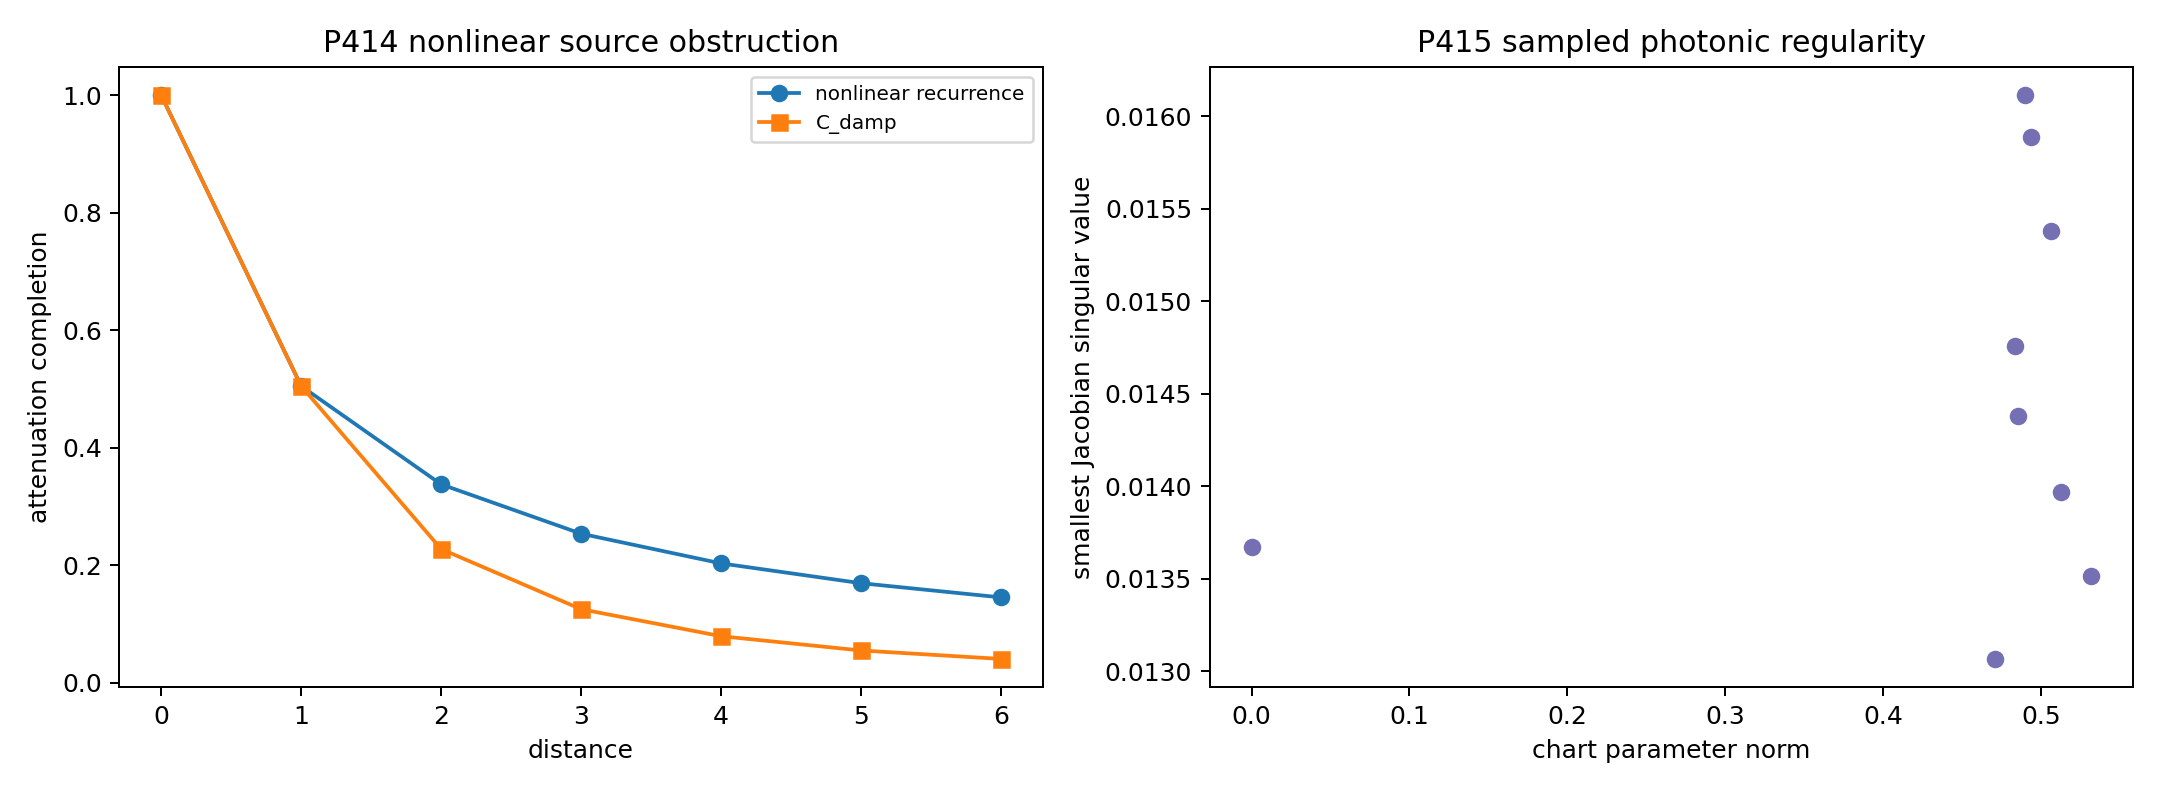
\includegraphics[width=0.97\textwidth]{FIN_Programs_411_427_Figures/p414_p415_damping_photonic.png}
\caption{The normalized nonlinear damping-source obstruction and sampled photonic Jacobian regularity.}
\end{figure}

\section{Physical boundary}

P416 remains closed. A real pilot must supply a calibrated complex-transfer record, apparatus description, phase reference, traceable clock, detector response, provider/\allowbreak{}registrar separation, frozen raw hash, and one-shot analysis. No such bundle is in the repository.

\chapter{P417 --- noisy-comb gap atlas}

P417 optimizes permutation-symmetric pure parallel inputs for \(n=2,3,4\) uses over a grid of coherence and time values. It compares the result with the adaptive hybrid upper bound

\[
D_n^{\rm adaptive}
\le\min\{1,nq|\sin\theta|\}.
\]

Three ideal-boundary rows close the gap numerically. Under genuine dephasing, the maximum remaining gap is approximately

\[
0.52763.
\]

The large residual gap is scientifically useful: the missing object is not another input ansatz but a semidefinite dual certificate or a counterexample adaptive strategy. The local environment contains no certified SDP solver, and nonlinear pure-state optimization cannot be relabelled as such a proof.

\chapter{P418 --- heralded-erasure-aware symmetric code}

\section{Construction}

Let an \(n\)-qubit permutation-symmetric input be parameterized by weights \(p_0,\ldots,p_n\) on Hamming sectors. Independent dephasing multiplies each matrix element by

\[
q^{d_H(a,b)}.
\]

For every heralded survivor set \(S\subseteq\{1,\ldots,n\}\), P418 computes

\[
\rho_S^\pm=\operatorname{Tr}_{S^c}\rho^\pm
\]

exactly in finite matrix arithmetic. Since survivor patterns are orthogonal classical records, the feasible discrimination value is

\[
D_{n,\eta,q}(p)
=\sum_S
\eta^{|S|}(1-\eta)^{n-|S|}
\frac12\|\rho_S^+-\rho_S^-\|_1.
\]

The sector law \(p\) is then optimized.

\section{Result}

For \(n\in\{3,4\}\), \(q\in\{0.6,0.8\}\), \(\eta\in\{0.6,0.8\}\), and two first-branch time fractions, the optimized code strictly exceeds both the product and GHZ baselines in all 16 cells. The largest gain is

\[
0.0269418715.
\]

This is the most constructive new operational result of the round.

\section{Boundary}

The search is numerical, uses \(n\le4\), and restricts amplitudes to the permutation-symmetric sector with a fixed phase convention. It does not prove global optimality, fault tolerance, or physical implementability.

\begin{figure}[htbp]
\centering
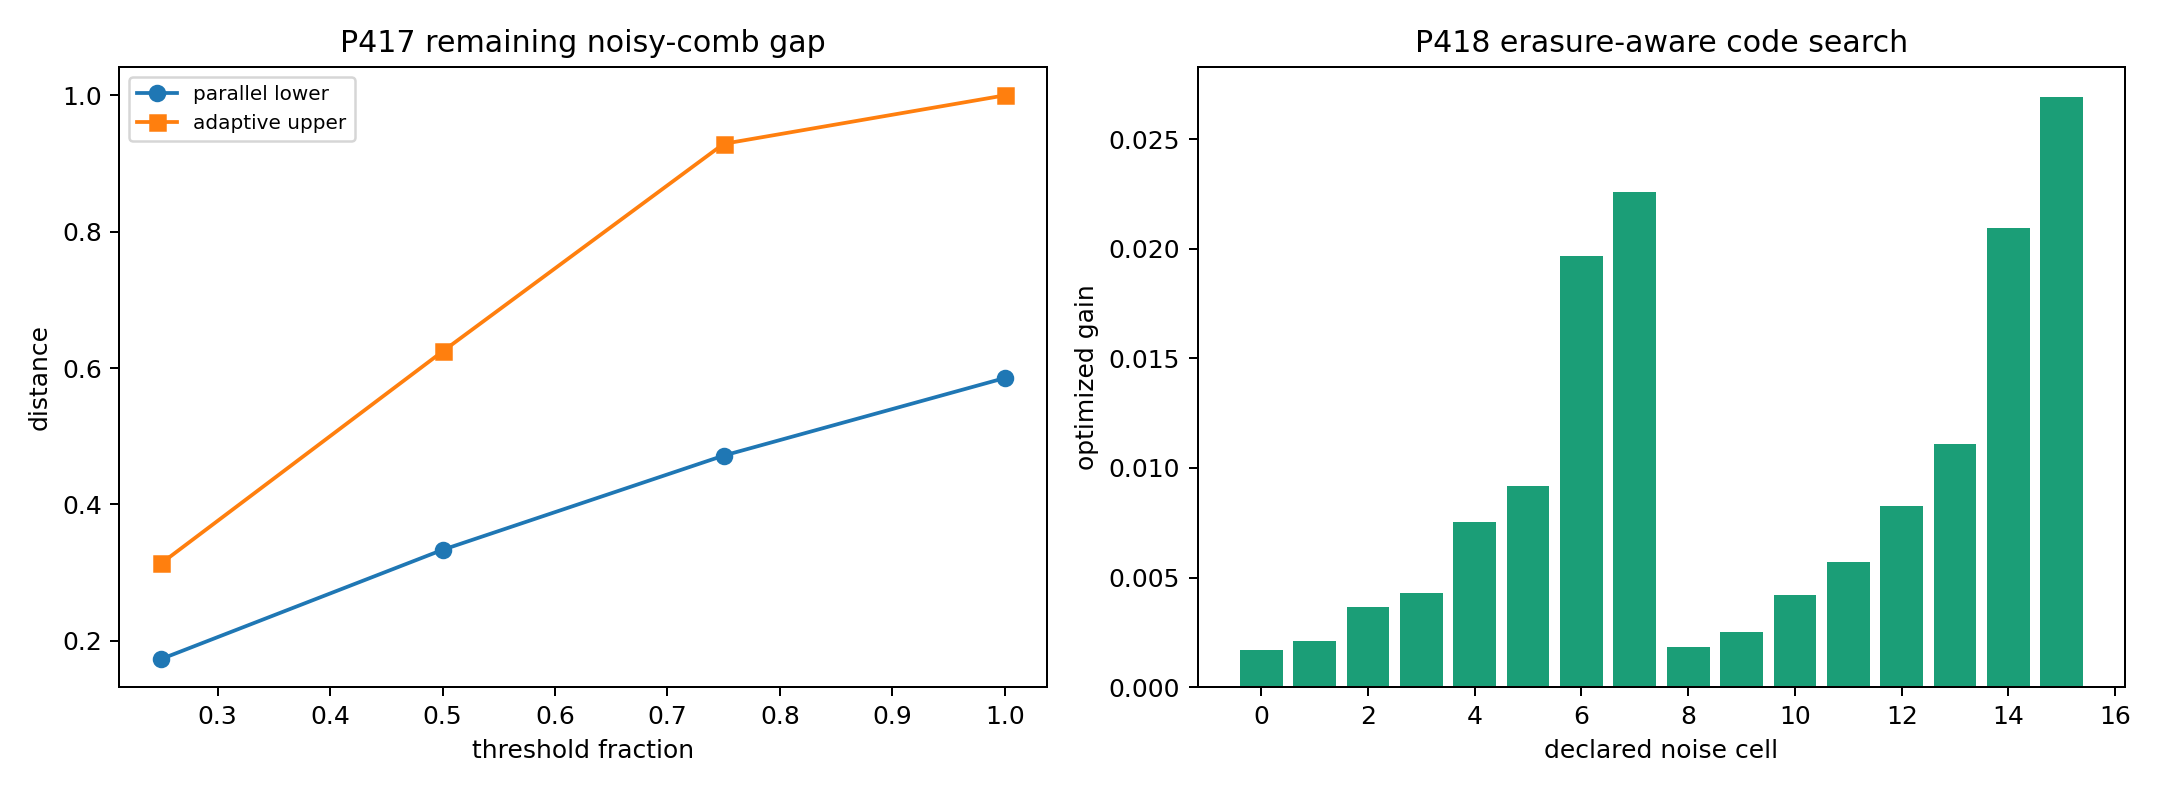
\includegraphics[width=0.97\textwidth]{FIN_Programs_411_427_Figures/p417_p418_noisy_erasure.png}
\caption{The remaining noisy-comb certificate gap and gains from the new heralded-erasure-aware symmetric code.}
\end{figure}

\chapter{P419 --- full twelve-mode one-use test}

The strict and amplitude-absorbed legacy comparison generators are circulant and share the Fourier basis to defect

\[
5.07\times10^{-15}.
\]

The relative-generator spectral diameter in the declared comparison is

\[
9.2871940587.
\]

P419 optimizes all twelve input probabilities for eight combinations of coherence, survival, and time. No tested row improves on the equal superposition of the two extremal relative-generator modes.

This is evidence that the one-use uniform-dephasing problem collapses to an extremal pair. It is not a proof for every time/\allowbreak{}noise point and does not extend to several adaptive uses, nonuniform dephasing, or noncommuting apparatus noise.

\chapter{P420--P421 --- the physical boundary remains real}

P420 requires a traceable map from laboratory SI time to the dimensionless FIN evolution parameter. No such clock anchor is present.

P421 requires external execution of the P403 Jordan Sampling Realization with independent provider, registrar, and analyst; a raw hash frozen before unblinding; real apparatus and calibration identifiers; and failure reporting without model repair. A synthetic event file can test a validator but cannot satisfy these obligations.

\chapter{P422 --- variance-optimal JSR estimator}

\section{Objective}

For atoms \((x_i,w_i)\), choose a positive sampling distribution \(q_i\). The unbiased estimator for moment \(k\) is

\[
Y_k(i)=\frac{w_i x_i^k}{q_i}.
\]

For equal loss on the twelve moments, the sum of second moments is

\[
\sum_i\frac{w_i^2}{q_i}
\left(\sum_{k=0}^{11}x_i^{2k}\right).
\]

\section{Theorem}

By Cauchy--Schwarz, the unique optimum on the positive simplex is

\[
\boxed{
q_i^\star=
\frac{|w_i|r_i}{\sum_j|w_j|r_j},
\qquad
r_i=\sqrt{\sum_{k=0}^{11}x_i^{2k}}.
}
\]

The estimator remains unbiased. For the frozen seven-atom certificate, the total declared variance changes from

\[
7.26544217
\quad\text{to}\quad
6.42447801,
\]

a reduction of

\[
11.5749\%.
\]

This is a theorem for the stated multi-moment loss, not a universal apparatus efficiency result.

\begin{figure}[htbp]
\centering
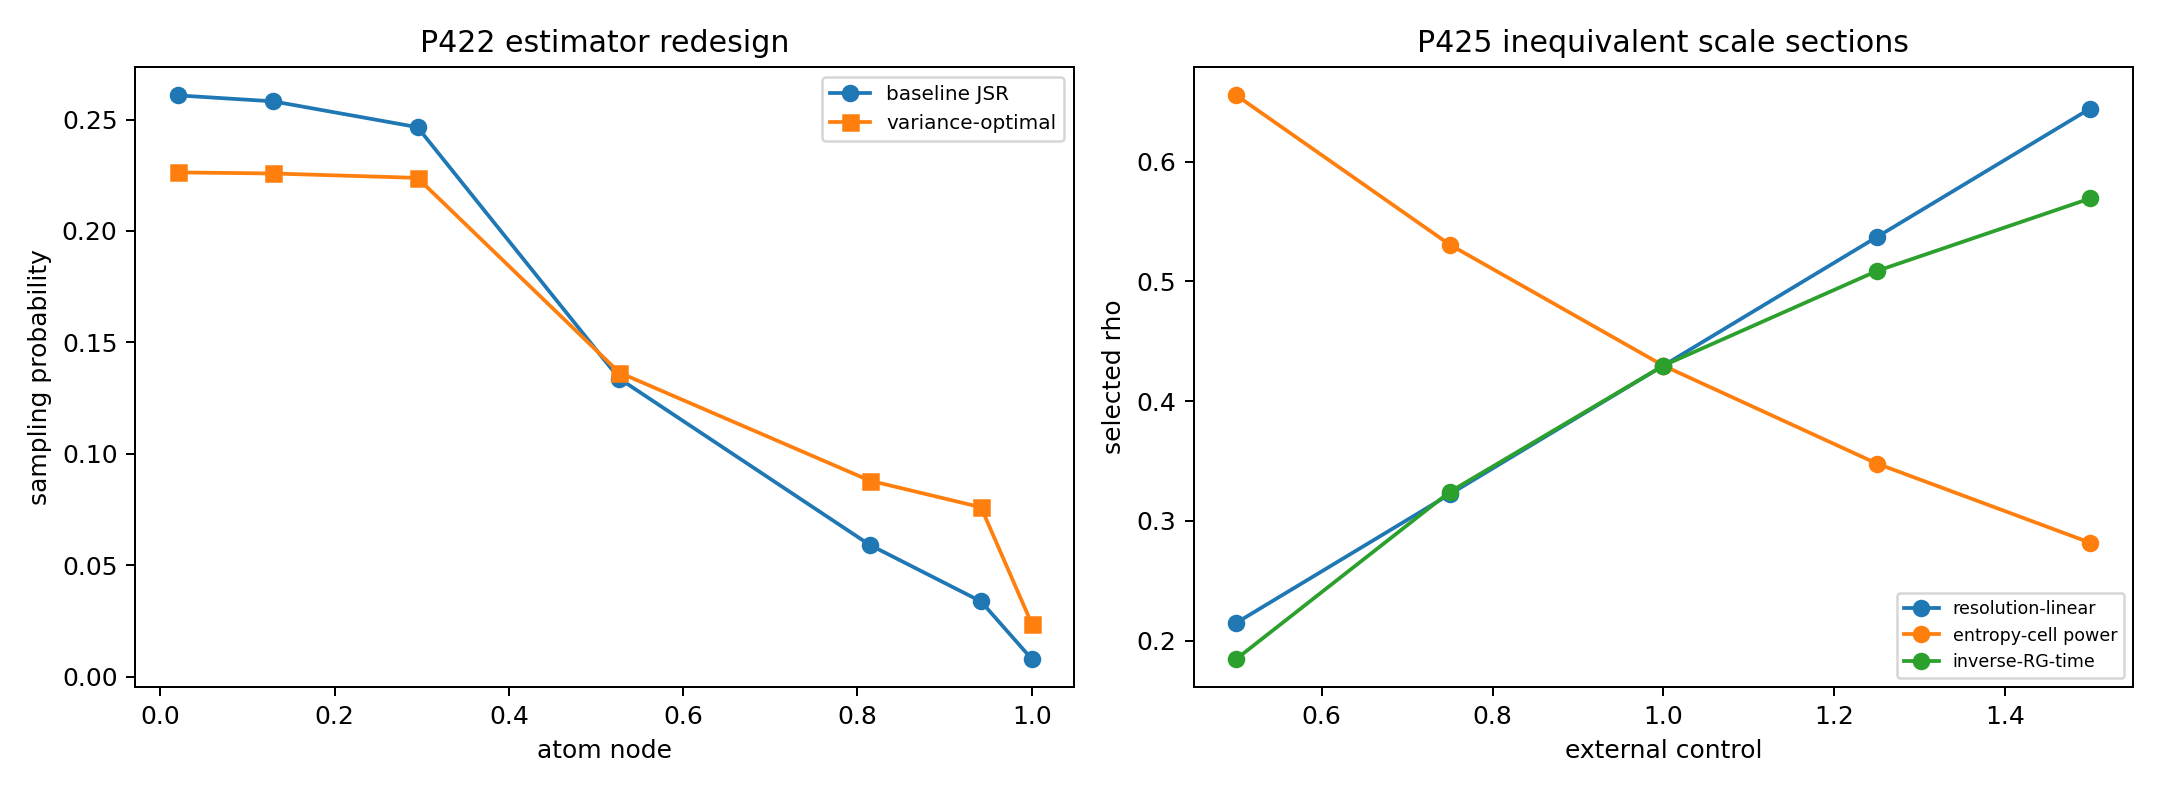
\includegraphics[width=0.97\textwidth]{FIN_Programs_411_427_Figures/p422_p425_estimator_scale.png}
\caption{Variance-optimal Jordan sampling and inequivalent conditional outer-scale sections.}
\end{figure}

\chapter{P423 --- phase-reference conversion ledger}

For negative-sign probability \(q_-\), the conditional coherent encoder

\[
s=+1\mapsto|+\rangle,
\qquad
s=-1\mapsto|-\rangle
\]

produces

\[
\rho(q_-)=
\frac12
\begin{pmatrix}
1&1-2q_-\\
1-2q_-&1
\end{pmatrix}.
\]

Therefore

\[
C_{l_1}(\rho)=|1-2q_-|,
\]

and its relative entropy of \(U(1)\) asymmetry is

\[
A(\rho)=1-H_2(q_-).
\]

A classical diagonal sign register cannot generate this coherence under \(U(1)\)-covariant incoherent operations. The chosen encoder consumes an aligned phase reference. Swapping the two phase labels reverses polarity but does not change any reported cost. Thus the conversion is conditional and does not select a strict orientation.

\chapter{P424 --- an explicit odd object and why it is not the selector}

\section{Oriented record current}

The seven-atom JSR object admits the explicit functional

\[
J_{\rm or}(w,x)
=\sum_iw_i\sin(2\pi x_i).
\]

Under reflection \(R:x\mapsto1-x\),

\[
J_{\rm or}(w,Rx)=-J_{\rm or}(w,x).
\]

For the frozen atoms,

\[
J_{\rm or}=0.7858270815460081,
\]

and the computed oddness defect is \(1.11\times10^{-16}\).

\section{Selector falsification}

This is a real inversion-odd observable, but its sign uses the declared chart orientation \(0\to1\). Reversing that coordinate flips the current. The strict radial kernel does not choose between these two charts. Consequently, the object is an oriented measurement receiver or record, not a strict non-premise source. QW-2191 remains open.

\chapter{P425 --- scale-section comparison}

P389 proved that dilation alone does not choose a positive outer scale. P425 normalizes three supplied sections to the same baseline

\[
\rho_0=0.4296970877901551
\]

at control \(u=1\):

\[
\rho_R(u)=\rho_0u,
\qquad
\rho_E(u)=\rho_0^u,
\qquad
\rho_G(u)=\exp\!\left(-\frac{-\log\rho_0}{u}\right).
\]

Their logarithmic derivatives at the common point are distinct:

\[
1,
\qquad
\log\rho_0,
\qquad
-\log\rho_0.
\]

Thus equality at one calibration point does not establish equivalence of the resolution, entropy-cell, and inverse-RG laws. Conversely, a nonlinear reparameterization of the external control can map any monotone section to another. Physical semantics for the control are therefore indispensable.

\chapter{P426--P427 --- external campaigns}

P426 combines three still-empty admission classes: an independent QW hold-out, traceable dimensional standards, and reservoir process tomography. No admissible external record is present.

P427 remains inadmissible for two independent reasons. First, there is no closed source-independent legacy-to-strict role-transfer theorem. Second, there is no frozen independent electroweak bundle with the required custody and unblinding chain. Reusing a historical target as both parameter source and test would be circular.

\chapter{Newly constructed theoretical objects}

\section{O143 --- Taylor Trust Lattice}

The typed chain

\[
\text{rational phase}
\to\text{exact Taylor arithmetic}
\to\text{analytic cosine bridge}
\to\text{moment interval}
\]

separates proof-kernel work from the one remaining analytic provider.

\section{O144 --- Simultaneous Contact Replacement Candidate}

A 25-dimensional primal-dual KKT object with seven contacts replaces the known noncomplementary frozen pair. It is numerical until interval certified.

\section{O145 --- Transcendence Provider Boundary}

The injectivity proof is factored into finite algebraic reduction and one named Lindemann--Weierstrass provider.

\section{O146 --- Nonlinear RG-Recurrence Obstruction}

An exact two-step integer contradiction excludes one state-nonlinear completion source without reopening the generic bridge.

\section{O147 --- Sampled Photonic Regularity Atlas}

A finite atlas records the smallest complex-transfer singular value and condition number at each tested chart point.

\section{O148 --- Noisy Comb Primal-Dual-Gap Atlas}

Each declared noise cell stores a feasible optimized parallel strategy, the analytic hybrid upper bound, and the unresolved certificate gap.

\section{O149 --- Heralded Erasure-Aware Symmetric Code}

This code retains every survivor pattern, traces lost subsystems, and optimizes Hamming-sector weights. It strictly improves the two prior baseline families on the declared grid.

\section{O150 --- Twelve-Mode Noise-Adapted Simplex}

The object is the probability simplex over all common Fourier modes equipped with one-use dephased trace-distance objective. The tested optimum lies on the extremal two-mode face.

\section{O151 --- Variance-Optimal JSR Sampling Law}

This is an exact positive-probability realization optimized for twelve simultaneous moments rather than only total variation.

\section{O152 --- Phase-Reference Conversion Ledger}

It records coherence/\allowbreak{}asymmetry output together with the explicitly consumed phase reference and the unresolved polarity convention.

\section{O153 --- Oriented JSR Record Current}

A nonzero inversion-odd receiver is constructed. Its convention dependence is part of its type and prevents selector overpromotion.

\section{O154 --- Conditional Scale-Section Comparison Groupoid}

Scale sections and reparameterizations of their external controls are kept separate. This exposes why numerical agreement at one point cannot establish canonical scale generation.

\chapter{Cross-program synthesis}

\section{What advanced}

Four fronts advanced materially:

\begin{enumerate}
\item 
the trusted arithmetic around strict cosine moments was reduced;

\item 
the geometry of the exact oscillatory optimizer acquired a concrete simultaneous-contact candidate;

\item 
noisy operational discrimination gained an erasure-aware code that beats both existing baselines;

\item 
the JSR protocol acquired an analytically optimal multi-moment sampler and a typed phase-reference ledger.

\end{enumerate}

\section{What was falsified}

The round falsifies three tempting shortcuts:

\begin{enumerate}
\item 
the declared nonlinear recurrence cannot source \(C_{\rm damp}\);

\item 
a nonzero inversion-odd record does not automatically source a canonical orientation;

\item 
agreeing scale laws at one normalization point do not become the same physical scale law.

\end{enumerate}

\section{Deepest surviving interpretation}

The strongest current interpretation remains:

\begin{quote}\itshape
FIN is a finite spectral-information and operational mathematics framework with several rigorously typed realizations and discrimination problems, but physical interpretation requires additional reference structures and independent records.

\end{quote}

The operator supplies wave and diffusion functional calculi. The additional objects that make an experiment meaningful --- preparation, clock, reference frame, environment, instrument, apparatus response, record, and dimensional anchor --- are not automatic shadows of the spectral theorem. P418 and P422 show that once such operational structure is declared, nontrivial and useful theorems follow. P423--P425 show that these declarations cannot be erased from the provenance after the fact.

\chapter{Recommended next programs P428--P444}

The next studies are ranked by the probability of a decisive result, including a rigorous obstruction.

\begin{center}
\begingroup\fontsize{7}{8.4}\selectfont
\setlength{\tabcolsep}{2.5pt}
\renewcommand{\arraystretch}{1.16}
\begin{longtable}{@{}p{0.055\textwidth}p{0.077\textwidth}p{0.328\textwidth}p{0.280\textwidth}p{0.120\textwidth}@{}}
\toprule
\textbf{Rank} & \textbf{Program} & \textbf{Study} & \textbf{Decisive output} & \textbf{Probability} \\
\midrule
\endhead
1 & \textbf{P429} & 25-variable interval Krawczyk/\allowbreak{}radii certificate for O144 & Certified local KKT existence and uniqueness, or a rigorous failure box & 0.72 \\
2 & \textbf{P428} & Formal analytic cosine bridge & Mathlib/\allowbreak{}Lean proof that the P411 Taylor sums bound real cosine at all twelve phases & 0.68 \\
3 & \textbf{P436} & Rigorous certification of the P418 code gain & Interval trace norms and globally certified simplex lower bounds in at least one noise cell & 0.66 \\
4 & \textbf{P440} & Minimax and apparatus-aware JSR estimator & Optimal law with detector efficiency, dark counts, and finite-sample confidence included & 0.64 \\
5 & \textbf{P430} & Exact global dual feasibility for O144 & Rational Bernstein certificate for \(-1\le p\le0\) with contact boxes & 0.61 \\
6 & \textbf{P435} & Noisy-comb SDP primal/\allowbreak{}dual implementation & Matching certified primal and dual within \(10^{-4}\) on one nonideal cell & 0.58 \\
7 & \textbf{P432} & One complete-Bernstein/\allowbreak{}subordination damping source class & Source-derived atom or exact order/\allowbreak{}convexity obstruction; one class only & 0.55 \\
8 & \textbf{P437} & Multi-use twelve-mode comb & Certified comparison of the extremal face with genuine multimode/\allowbreak{}adaptive strategies & 0.50 \\
9 & \textbf{P433} & Interval cover of the photonic chart & Nonsingular cover of a nontrivial box or an explicit compensating alias & 0.46 \\
10 & \textbf{P441} & Catalytic phase-reference conversion rate & Exact reference consumption/\allowbreak{}recovery law and polarity nonpromotion theorem & 0.45 \\
11 & \textbf{P442} & Representation-independence audit of O153 & Determine whether any odd record survives support change, relabeling, and JSR nonuniqueness & 0.42 \\
12 & \textbf{P443} & Operational semantics for one scale section & One traceably calibrated external control with preregistered response law & 0.35 \\
13 & \textbf{P431} & Full formal Lindemann--Weierstrass import & Kernel-checked P381 injectivity without the P413 analytic axiom & 0.30 \\
14 & \textbf{P434} & Independent photonic pilot & Calibrated complex-transfer record with provider/\allowbreak{}registrar separation & 0.28 \\
15 & \textbf{P438} & Traceable clock execution & Frozen SI-to-\(\tau\) map and uncertainty-propagated P418/\allowbreak{}P419 schedule & 0.25 \\
16 & \textbf{P439} & External JSR run & Physical event record passing the frozen executable validator without repair & 0.25 \\
17 & \textbf{P444} & Combined QW/\allowbreak{}standards/\allowbreak{}reservoir/\allowbreak{}EW admission gate & At least one external admission; EW remains conditional on role-source closure & 0.12 \\
\bottomrule
\end{longtable}
\endgroup
\end{center}

\section{Preferred sequence}

The recommended immediate sequence is

\[
\boxed{
P428\to P429\to P430\to P435\to P436\to P440.
}
\]

P428 reduces the formal trust boundary. P429--P430 determine whether the simultaneous KKT candidate becomes a theorem. P435 attacks the largest remaining noisy-comb gap. P436 certifies the most promising new constructive strategy. P440 converts the mathematical JSR improvement into a design that can incorporate a real detector model.

P432 must test only one explicitly declared subordination class. P442 must not promote an oriented record to a strict selector unless orientation survives representation change without a supplied chart. External Programs P434/\allowbreak{}P438/\allowbreak{}P439/\allowbreak{}P443/\allowbreak{}P444 cannot be completed by repository-generated data.

\chapter{Reproducibility}

Run:

``bash MPLCONFIGDIR=/\allowbreak{}tmp/\allowbreak{}mpl-fin-1035 \\
python3 fin\_programs\_411\_427.py

python3 -m unittest -v test\_fin\_programs\_411\_427.py `

Expected result: 16 tests passed, zero failed. The Lean 4.28 Taylor source must compile. The random seed is 20260766`. Exact arithmetic is used for the Taylor sums and the nonlinear recurrence obstruction. Floating-point linear algebra and nonlinear optimization are used for P412, P415, P417--P419 and are labelled as strong evidence rather than proof.

\chapter{Final conclusion}

P411--P427 do not supply a missing universal theorem that converts the FIN operator into physics. They provide a sharper and more useful result.

The mathematical core continues to support exact spectral, variational, moment, wave, diffusion, and information-processing constructions. The new erasure-aware code shows that operational structure can generate genuinely new predictions beyond the bare product/\allowbreak{}GHZ dichotomy. The optimal JSR sampler shows that the signed representation can be turned into a better positive-data experiment without interpreting its sign as negative probability.

At the same time, every attempted shortcut to the missing physical bridge fails cleanly. Nonlinear recurrence does not source the damping atom. An odd record does not choose its own orientation. A phase encoding consumes a phase reference. A scale section consumes a control law. A clock and a laboratory record remain external.

The deepest interpretation surviving this round is therefore not that one spectral operator already contains all of physics. It is that the operator is the stable mathematical core of a family of operational models, while the passage to experimentally testable physics is a typed extension problem. The shortest path forward is to certify O144 and O149 mathematically, then attach one independently calibrated clock, reference frame, apparatus model, and raw event record without changing the frozen theory after unblinding.


\clearpage
\chapter*{Reproduction certificate}
\addcontentsline{toc}{chapter}{Reproduction certificate}
\begin{Verbatim}[fontsize=\small]
MPLCONFIGDIR=/tmp/mpl-fin-1035 \
python3 fin_programs_411_427.py

python3 -m unittest -v test_fin_programs_411_427.py
\end{Verbatim}
Expected result: 16 tests passed, zero failed. P416, P420, P421, P426, and
P427 remain external gates. Synthetic or repository-generated records are
not accepted as physical evidence.

\medskip
\noindent\textbf{Suggested citation:}

\.Zuchowski, K. (2026). \emph{FIN Research Programs P411--P427: Formal Cosine
Boundary, Simultaneous Contact Geometry, Erasure-Aware Discrimination, and
Operational Reference Resources} (Release 10.35; Version 1.0.0) [Preprint].
Zenodo.

\end{document}
